\begin{figure}[!h]
\centering
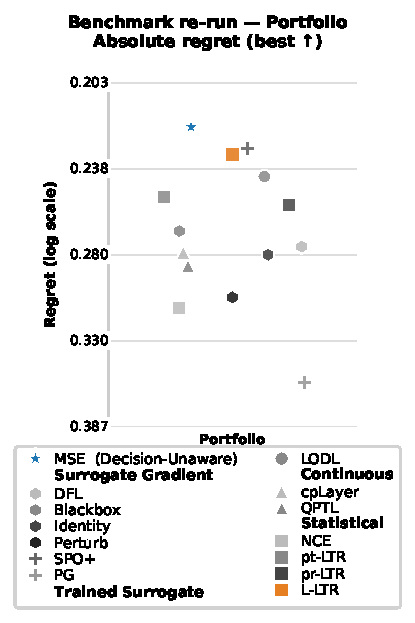
\includegraphics[height=10cm]{figures/fig_bench_bump_portfolio.pdf}

% Tighten space before caption (local to this figure)
\vspace{-0.3em}
\setlength{\abovecaptionskip}{2pt}
\setlength{\belowcaptionskip}{0pt}
\caption[Comparison of decision-aware learning methods on the Portfolio task.]{
\textbf{Portfolio Task}
The Portfolio task is not a combinatorial optimization problem, and again we see strong performance from decision-unaware methods. We also plot a decision-focused learning solution which directly optimizes the decision loss; the label ``DFL'' in this figure refers to this generic decision-focused learning approach in the sense of \citet{shahDecisionFocusedLearningDifferentiable2022}, distinct from ``DFL by Wilder et al.\ '' shown in the Budget figure above.
}%endcaption
\label{fig:portfolio_bump}
\end{figure}
